% Created by tikzDevice version 0.10.1 on 2017-02-16 15:14:47
% !TEX encoding = UTF-8 Unicode
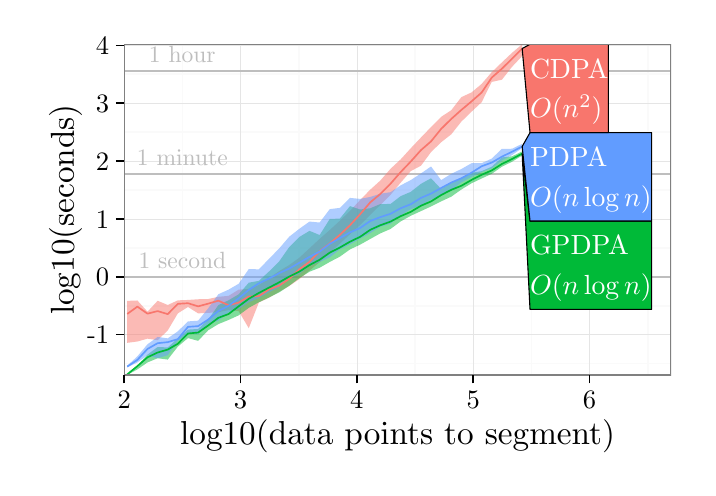
\begin{tikzpicture}[x=1pt,y=1pt]
\definecolor{fillColor}{RGB}{255,255,255}
\path[use as bounding box,fill=fillColor,fill opacity=0.00] (0,0) rectangle (238.49,158.99);
\begin{scope}
\path[clip] (  0.00,  0.00) rectangle (238.49,158.99);
\definecolor{drawColor}{RGB}{255,255,255}
\definecolor{fillColor}{RGB}{255,255,255}

\path[draw=drawColor,line width= 0.6pt,line join=round,line cap=round,fill=fillColor] (  0.00,  0.00) rectangle (238.49,158.99);
\end{scope}
\begin{scope}
\path[clip] ( 34.86, 33.48) rectangle (232.49,152.99);
\definecolor{fillColor}{RGB}{255,255,255}

\path[fill=fillColor] ( 34.86, 33.48) rectangle (232.49,152.99);
\definecolor{drawColor}{gray}{0.98}

\path[draw=drawColor,line width= 0.6pt,line join=round] ( 34.86, 37.63) --
	(232.49, 37.63);

\path[draw=drawColor,line width= 0.6pt,line join=round] ( 34.86, 58.53) --
	(232.49, 58.53);

\path[draw=drawColor,line width= 0.6pt,line join=round] ( 34.86, 79.43) --
	(232.49, 79.43);

\path[draw=drawColor,line width= 0.6pt,line join=round] ( 34.86,100.33) --
	(232.49,100.33);

\path[draw=drawColor,line width= 0.6pt,line join=round] ( 34.86,121.23) --
	(232.49,121.23);

\path[draw=drawColor,line width= 0.6pt,line join=round] ( 34.86,142.13) --
	(232.49,142.13);

\path[draw=drawColor,line width= 0.6pt,line join=round] ( 55.89, 33.48) --
	( 55.89,152.99);

\path[draw=drawColor,line width= 0.6pt,line join=round] ( 97.94, 33.48) --
	( 97.94,152.99);

\path[draw=drawColor,line width= 0.6pt,line join=round] (139.98, 33.48) --
	(139.98,152.99);

\path[draw=drawColor,line width= 0.6pt,line join=round] (182.03, 33.48) --
	(182.03,152.99);

\path[draw=drawColor,line width= 0.6pt,line join=round] (224.08, 33.48) --
	(224.08,152.99);
\definecolor{drawColor}{gray}{0.90}

\path[draw=drawColor,line width= 0.2pt,line join=round] ( 34.86, 48.08) --
	(232.49, 48.08);

\path[draw=drawColor,line width= 0.2pt,line join=round] ( 34.86, 68.98) --
	(232.49, 68.98);

\path[draw=drawColor,line width= 0.2pt,line join=round] ( 34.86, 89.88) --
	(232.49, 89.88);

\path[draw=drawColor,line width= 0.2pt,line join=round] ( 34.86,110.78) --
	(232.49,110.78);

\path[draw=drawColor,line width= 0.2pt,line join=round] ( 34.86,131.68) --
	(232.49,131.68);

\path[draw=drawColor,line width= 0.2pt,line join=round] ( 34.86,152.58) --
	(232.49,152.58);

\path[draw=drawColor,line width= 0.2pt,line join=round] ( 34.86, 33.48) --
	( 34.86,152.99);

\path[draw=drawColor,line width= 0.2pt,line join=round] ( 76.91, 33.48) --
	( 76.91,152.99);

\path[draw=drawColor,line width= 0.2pt,line join=round] (118.96, 33.48) --
	(118.96,152.99);

\path[draw=drawColor,line width= 0.2pt,line join=round] (161.01, 33.48) --
	(161.01,152.99);

\path[draw=drawColor,line width= 0.2pt,line join=round] (203.06, 33.48) --
	(203.06,152.99);
\definecolor{drawColor}{RGB}{190,190,190}

\path[draw=drawColor,line width= 0.6pt,line join=round] ( 34.86, 68.98) -- (232.49, 68.98);

\path[draw=drawColor,line width= 0.6pt,line join=round] ( 34.86,106.15) -- (232.49,106.15);

\path[draw=drawColor,line width= 0.6pt,line join=round] ( 34.86,143.31) -- (232.49,143.31);
\definecolor{fillColor}{RGB}{248,118,109}

\path[fill=fillColor,fill opacity=0.50] ( 35.98, 60.27) --
	( 39.64, 60.41) --
	( 43.30, 56.36) --
	( 46.96, 60.30) --
	( 50.61, 58.78) --
	( 54.27, 60.46) --
	( 57.93, 60.60) --
	( 61.59, 60.85) --
	( 65.25, 60.94) --
	( 68.91, 61.74) --
	( 72.57, 62.07) --
	( 76.23, 64.32) --
	( 79.89, 64.59) --
	( 83.55, 66.01) --
	( 87.20, 68.46) --
	( 90.86, 71.05) --
	( 94.52, 73.24) --
	( 98.18, 75.89) --
	(101.84, 79.27) --
	(105.50, 82.68) --
	(109.16, 85.88) --
	(112.82, 89.24) --
	(116.48, 92.77) --
	(120.14, 96.72) --
	(123.79,100.45) --
	(127.45,103.76) --
	(131.11,107.98) --
	(134.77,111.39) --
	(138.43,115.41) --
	(142.09,119.27) --
	(145.75,123.07) --
	(149.41,126.76) --
	(153.07,129.17) --
	(156.72,133.89) --
	(160.38,135.58) --
	(164.04,138.67) --
	(167.70,142.92) --
	(171.36,146.44) --
	(175.02,149.89) --
	(178.68,152.99) --
	(178.68,148.74) --
	(175.02,144.85) --
	(171.36,140.19) --
	(167.70,139.39) --
	(164.04,132.05) --
	(160.38,128.63) --
	(156.72,125.06) --
	(153.07,120.46) --
	(149.41,117.59) --
	(145.75,114.03) --
	(142.09,109.09) --
	(138.43,107.16) --
	(134.77,102.98) --
	(131.11, 98.57) --
	(127.45, 94.95) --
	(123.79, 91.35) --
	(120.14, 87.71) --
	(116.48, 84.32) --
	(112.82, 80.95) --
	(109.16, 77.70) --
	(105.50, 74.27) --
	(101.84, 71.22) --
	( 98.18, 68.16) --
	( 94.52, 65.64) --
	( 90.86, 63.56) --
	( 87.20, 61.39) --
	( 83.55, 59.71) --
	( 79.89, 50.40) --
	( 76.23, 56.58) --
	( 72.57, 56.93) --
	( 68.91, 56.18) --
	( 65.25, 55.92) --
	( 61.59, 55.76) --
	( 57.93, 58.06) --
	( 54.27, 55.76) --
	( 50.61, 49.59) --
	( 46.96, 46.06) --
	( 43.30, 46.61) --
	( 39.64, 45.59) --
	( 35.98, 45.10) --
	cycle;
\definecolor{fillColor}{RGB}{0,186,56}

\path[fill=fillColor,fill opacity=0.50] ( 35.98, 33.92) --
	( 39.64, 36.85) --
	( 43.30, 40.84) --
	( 46.96, 43.60) --
	( 50.61, 43.45) --
	( 54.27, 46.72) --
	( 57.93, 49.89) --
	( 61.59, 50.11) --
	( 65.25, 53.52) --
	( 68.91, 58.73) --
	( 72.57, 60.48) --
	( 76.23, 62.62) --
	( 79.89, 66.84) --
	( 83.55, 67.50) --
	( 87.20, 70.88) --
	( 90.86, 74.51) --
	( 94.52, 79.72) --
	( 98.18, 83.37) --
	(101.84, 85.57) --
	(105.50, 84.06) --
	(109.16, 89.85) --
	(112.82, 90.02) --
	(116.48, 94.51) --
	(120.14, 93.29) --
	(123.79, 93.73) --
	(127.45, 95.26) --
	(131.11, 95.28) --
	(134.77, 98.11) --
	(138.43, 99.66) --
	(142.09,102.55) --
	(145.75,104.57) --
	(149.41,100.67) --
	(153.07,103.01) --
	(156.72,104.80) --
	(160.38,106.57) --
	(164.04,107.14) --
	(167.70,108.75) --
	(171.36,112.11) --
	(175.02,112.51) --
	(178.68,114.26) --
	(178.68,112.81) --
	(175.02,110.53) --
	(171.36,108.75) --
	(167.70,106.19) --
	(164.04,104.49) --
	(160.38,102.75) --
	(156.72,100.52) --
	(153.07, 97.92) --
	(149.41, 96.23) --
	(145.75, 94.38) --
	(142.09, 92.70) --
	(138.43, 91.01) --
	(134.77, 88.97) --
	(131.11, 86.25) --
	(127.45, 84.67) --
	(123.79, 82.64) --
	(120.14, 80.59) --
	(116.48, 78.87) --
	(112.82, 76.25) --
	(109.16, 74.34) --
	(105.50, 72.25) --
	(101.84, 70.80) --
	( 98.18, 68.50) --
	( 94.52, 65.75) --
	( 90.86, 63.32) --
	( 87.20, 61.49) --
	( 83.55, 59.76) --
	( 79.89, 57.75) --
	( 76.23, 55.03) --
	( 72.57, 53.37) --
	( 68.91, 51.88) --
	( 65.25, 49.66) --
	( 61.59, 45.83) --
	( 57.93, 46.82) --
	( 54.27, 43.75) --
	( 50.61, 39.06) --
	( 46.96, 39.54) --
	( 43.30, 38.02) --
	( 39.64, 35.50) --
	( 35.98, 33.48) --
	cycle;
\definecolor{fillColor}{RGB}{97,156,255}

\path[fill=fillColor,fill opacity=0.50] ( 35.98, 36.85) --
	( 39.64, 40.21) --
	( 43.30, 44.58) --
	( 46.96, 47.23) --
	( 50.61, 46.72) --
	( 54.27, 49.27) --
	( 57.93, 52.85) --
	( 61.59, 53.11) --
	( 65.25, 57.59) --
	( 68.91, 62.66) --
	( 72.57, 64.32) --
	( 76.23, 66.44) --
	( 79.89, 71.75) --
	( 83.55, 71.67) --
	( 87.20, 75.45) --
	( 90.86, 79.18) --
	( 94.52, 83.46) --
	( 98.18, 86.32) --
	(101.84, 88.92) --
	(105.50, 88.58) --
	(109.16, 93.41) --
	(112.82, 93.88) --
	(116.48, 97.47) --
	(120.14, 97.12) --
	(123.79, 97.83) --
	(127.45, 98.98) --
	(131.11, 99.54) --
	(134.77,102.00) --
	(138.43,103.91) --
	(142.09,106.30) --
	(145.75,108.83) --
	(149.41,103.91) --
	(153.07,106.18) --
	(156.72,107.92) --
	(160.38,110.00) --
	(164.04,110.03) --
	(167.70,111.69) --
	(171.36,115.21) --
	(175.02,115.24) --
	(178.68,117.01) --
	(178.68,115.48) --
	(175.02,112.93) --
	(171.36,111.01) --
	(167.70,108.14) --
	(164.04,106.91) --
	(160.38,105.05) --
	(156.72,103.09) --
	(153.07,100.21) --
	(149.41, 98.37) --
	(145.75, 96.82) --
	(142.09, 94.83) --
	(138.43, 93.38) --
	(134.77, 91.15) --
	(131.11, 88.16) --
	(127.45, 87.10) --
	(123.79, 84.76) --
	(120.14, 82.79) --
	(116.48, 80.70) --
	(112.82, 78.91) --
	(109.16, 76.00) --
	(105.50, 74.32) --
	(101.84, 72.88) --
	( 98.18, 70.08) --
	( 94.52, 68.25) --
	( 90.86, 65.14) --
	( 87.20, 63.36) --
	( 83.55, 61.32) --
	( 79.89, 59.76) --
	( 76.23, 57.30) --
	( 72.57, 56.07) --
	( 68.91, 53.11) --
	( 65.25, 52.00) --
	( 61.59, 48.26) --
	( 57.93, 48.35) --
	( 54.27, 45.83) --
	( 50.61, 40.63) --
	( 46.96, 39.54) --
	( 43.30, 40.63) --
	( 39.64, 38.02) --
	( 35.98, 36.20) --
	cycle;
\definecolor{drawColor}{RGB}{248,118,109}

\path[draw=drawColor,line width= 0.6pt,line join=round] ( 35.98, 55.54) --
	( 39.64, 58.19) --
	( 43.30, 55.64) --
	( 46.96, 56.58) --
	( 50.61, 55.48) --
	( 54.27, 59.19) --
	( 57.93, 59.42) --
	( 61.59, 58.29) --
	( 65.25, 59.27) --
	( 68.91, 60.34) --
	( 72.57, 58.71) --
	( 76.23, 59.63) --
	( 79.89, 61.88) --
	( 83.55, 61.98) --
	( 87.20, 64.42) --
	( 90.86, 65.76) --
	( 94.52, 68.24) --
	( 98.18, 71.71) --
	(101.84, 74.39) --
	(105.50, 78.26) --
	(109.16, 81.00) --
	(112.82, 84.16) --
	(116.48, 87.61) --
	(120.14, 91.59) --
	(123.79, 95.87) --
	(127.45, 98.91) --
	(131.11,102.60) --
	(134.77,106.80) --
	(138.43,110.62) --
	(142.09,114.72) --
	(145.75,117.90) --
	(149.41,122.41) --
	(153.07,126.01) --
	(156.72,129.27) --
	(160.38,132.34) --
	(164.04,135.56) --
	(167.70,140.95) --
	(171.36,144.17) --
	(175.02,147.75) --
	(178.68,151.44);
\definecolor{drawColor}{RGB}{0,186,56}

\path[draw=drawColor,line width= 0.6pt,line join=round] ( 35.98, 33.70) --
	( 39.64, 36.69) --
	( 43.30, 39.88) --
	( 46.96, 41.61) --
	( 50.61, 42.66) --
	( 54.27, 44.78) --
	( 57.93, 48.48) --
	( 61.59, 48.82) --
	( 65.25, 51.39) --
	( 68.91, 54.15) --
	( 72.57, 55.50) --
	( 76.23, 58.29) --
	( 79.89, 61.02) --
	( 83.55, 63.14) --
	( 87.20, 65.05) --
	( 90.86, 66.96) --
	( 94.52, 69.05) --
	( 98.18, 70.84) --
	(101.84, 73.20) --
	(105.50, 75.13) --
	(109.16, 77.69) --
	(112.82, 79.55) --
	(116.48, 81.66) --
	(120.14, 83.42) --
	(123.79, 85.94) --
	(127.45, 87.60) --
	(131.11, 88.91) --
	(134.77, 90.87) --
	(138.43, 92.44) --
	(142.09, 94.64) --
	(145.75, 96.20) --
	(149.41, 98.50) --
	(153.07,100.40) --
	(156.72,101.87) --
	(160.38,103.97) --
	(164.04,105.84) --
	(167.70,107.41) --
	(171.36,109.74) --
	(175.02,111.53) --
	(178.68,113.49);
\definecolor{drawColor}{RGB}{97,156,255}

\path[draw=drawColor,line width= 0.6pt,line join=round] ( 35.98, 36.53) --
	( 39.64, 38.94) --
	( 43.30, 42.90) --
	( 46.96, 44.98) --
	( 50.61, 45.35) --
	( 54.27, 46.45) --
	( 57.93, 50.88) --
	( 61.59, 51.14) --
	( 65.25, 53.52) --
	( 68.91, 56.65) --
	( 72.57, 58.46) --
	( 76.23, 61.21) --
	( 79.89, 64.23) --
	( 83.55, 66.61) --
	( 87.20, 68.34) --
	( 90.86, 70.27) --
	( 94.52, 71.94) --
	( 98.18, 74.03) --
	(101.84, 76.17) --
	(105.50, 78.08) --
	(109.16, 80.86) --
	(112.82, 82.95) --
	(116.48, 85.03) --
	(120.14, 86.61) --
	(123.79, 89.13) --
	(127.45, 90.54) --
	(131.11, 91.73) --
	(134.77, 93.74) --
	(138.43, 95.19) --
	(142.09, 97.47) --
	(145.75, 99.04) --
	(149.41,101.05) --
	(153.07,103.03) --
	(156.72,104.57) --
	(160.38,106.58) --
	(164.04,108.91) --
	(167.70,110.25) --
	(171.36,112.37) --
	(175.02,114.16) --
	(178.68,116.05);
\definecolor{drawColor}{RGB}{190,190,190}

\node[text=drawColor,anchor=base,inner sep=0pt, outer sep=0pt, scale=  0.85] at ( 55.89, 71.92) {1 second};

\node[text=drawColor,anchor=base,inner sep=0pt, outer sep=0pt, scale=  0.85] at ( 55.89,109.09) {1 minute};

\node[text=drawColor,anchor=base,inner sep=0pt, outer sep=0pt, scale=  0.85] at ( 55.89,146.25) {1 hour};
\end{scope}
\begin{scope}
\path[clip] ( 34.86, 33.48) rectangle (232.49,152.99);
\definecolor{drawColor}{RGB}{0,0,0}
\definecolor{fillColor}{RGB}{0,186,56}

\path[draw=drawColor,line width= 0.4pt,line join=round,line cap=round,fill=fillColor] (178.68,113.49) --
	(181.52, 89.13) --
	(225.46, 89.13) --
	(225.46, 57.20) --
	(181.52, 57.20) --
	cycle;
\definecolor{fillColor}{RGB}{97,156,255}

\path[draw=drawColor,line width= 0.4pt,line join=round,line cap=round,fill=fillColor] (178.68,116.05) --
	(181.52,121.06) --
	(225.46,121.06) --
	(225.46, 89.13) --
	(181.52, 89.13) --
	cycle;
\definecolor{fillColor}{RGB}{248,118,109}

\path[draw=drawColor,line width= 0.4pt,line join=round,line cap=round,fill=fillColor] (178.68,151.44) --
	(181.52,152.99) --
	(209.85,152.99) --
	(209.85,121.06) --
	(181.52,121.06) --
	cycle;
\definecolor{drawColor}{RGB}{255,255,255}

\node[text=drawColor,anchor=base west,inner sep=0pt, outer sep=0pt, scale=  1.00] at (181.52, 76.92) {GPDPA};

\node[text=drawColor,anchor=base west,inner sep=0pt, outer sep=0pt, scale=  1.00] at (181.52, 62.52) {$O(n \log n)$};

\node[text=drawColor,anchor=base west,inner sep=0pt, outer sep=0pt, scale=  1.00] at (181.52,108.85) {PDPA};

\node[text=drawColor,anchor=base west,inner sep=0pt, outer sep=0pt, scale=  1.00] at (181.52, 94.45) {$O(n \log n)$};

\node[text=drawColor,anchor=base west,inner sep=0pt, outer sep=0pt, scale=  1.00] at (181.52,140.79) {CDPA};

\node[text=drawColor,anchor=base west,inner sep=0pt, outer sep=0pt, scale=  1.00] at (181.52,126.39) {$O(n^2)$};
\definecolor{drawColor}{gray}{0.50}

\path[draw=drawColor,line width= 0.6pt,line join=round,line cap=round] ( 34.86, 33.48) rectangle (232.49,152.99);
\end{scope}
\begin{scope}
\path[clip] (  0.00,  0.00) rectangle (238.49,158.99);
\definecolor{drawColor}{RGB}{0,0,0}

\node[text=drawColor,anchor=base east,inner sep=0pt, outer sep=0pt, scale=  0.96] at ( 29.46, 44.78) {-1};

\node[text=drawColor,anchor=base east,inner sep=0pt, outer sep=0pt, scale=  0.96] at ( 29.46, 65.68) {0};

\node[text=drawColor,anchor=base east,inner sep=0pt, outer sep=0pt, scale=  0.96] at ( 29.46, 86.58) {1};

\node[text=drawColor,anchor=base east,inner sep=0pt, outer sep=0pt, scale=  0.96] at ( 29.46,107.48) {2};

\node[text=drawColor,anchor=base east,inner sep=0pt, outer sep=0pt, scale=  0.96] at ( 29.46,128.38) {3};

\node[text=drawColor,anchor=base east,inner sep=0pt, outer sep=0pt, scale=  0.96] at ( 29.46,149.27) {4};
\end{scope}
\begin{scope}
\path[clip] (  0.00,  0.00) rectangle (238.49,158.99);
\definecolor{drawColor}{RGB}{0,0,0}

\path[draw=drawColor,line width= 0.6pt,line join=round] ( 31.86, 48.08) --
	( 34.86, 48.08);

\path[draw=drawColor,line width= 0.6pt,line join=round] ( 31.86, 68.98) --
	( 34.86, 68.98);

\path[draw=drawColor,line width= 0.6pt,line join=round] ( 31.86, 89.88) --
	( 34.86, 89.88);

\path[draw=drawColor,line width= 0.6pt,line join=round] ( 31.86,110.78) --
	( 34.86,110.78);

\path[draw=drawColor,line width= 0.6pt,line join=round] ( 31.86,131.68) --
	( 34.86,131.68);

\path[draw=drawColor,line width= 0.6pt,line join=round] ( 31.86,152.58) --
	( 34.86,152.58);
\end{scope}
\begin{scope}
\path[clip] (  0.00,  0.00) rectangle (238.49,158.99);
\definecolor{drawColor}{RGB}{0,0,0}

\path[draw=drawColor,line width= 0.6pt,line join=round] ( 34.86, 30.48) --
	( 34.86, 33.48);

\path[draw=drawColor,line width= 0.6pt,line join=round] ( 76.91, 30.48) --
	( 76.91, 33.48);

\path[draw=drawColor,line width= 0.6pt,line join=round] (118.96, 30.48) --
	(118.96, 33.48);

\path[draw=drawColor,line width= 0.6pt,line join=round] (161.01, 30.48) --
	(161.01, 33.48);

\path[draw=drawColor,line width= 0.6pt,line join=round] (203.06, 30.48) --
	(203.06, 33.48);
\end{scope}
\begin{scope}
\path[clip] (  0.00,  0.00) rectangle (238.49,158.99);
\definecolor{drawColor}{RGB}{0,0,0}

\node[text=drawColor,anchor=base,inner sep=0pt, outer sep=0pt, scale=  0.96] at ( 34.86, 21.46) {2};

\node[text=drawColor,anchor=base,inner sep=0pt, outer sep=0pt, scale=  0.96] at ( 76.91, 21.46) {3};

\node[text=drawColor,anchor=base,inner sep=0pt, outer sep=0pt, scale=  0.96] at (118.96, 21.46) {4};

\node[text=drawColor,anchor=base,inner sep=0pt, outer sep=0pt, scale=  0.96] at (161.01, 21.46) {5};

\node[text=drawColor,anchor=base,inner sep=0pt, outer sep=0pt, scale=  0.96] at (203.06, 21.46) {6};
\end{scope}
\begin{scope}
\path[clip] (  0.00,  0.00) rectangle (238.49,158.99);
\definecolor{drawColor}{RGB}{0,0,0}

\node[text=drawColor,anchor=base,inner sep=0pt, outer sep=0pt, scale=  1.20] at (133.68,  8.40) {log10(data points to segment)};
\end{scope}
\begin{scope}
\path[clip] (  0.00,  0.00) rectangle (238.49,158.99);
\definecolor{drawColor}{RGB}{0,0,0}

\node[text=drawColor,rotate= 90.00,anchor=base,inner sep=0pt, outer sep=0pt, scale=  1.20] at ( 16.66, 93.24) {log10(seconds)};
\end{scope}
\end{tikzpicture}
